\chapter{Spin, Isospin, Color, and Gluon Self-Interaction}

\section{Quantum Chromodynamics by Analogy with Electrodynamics}

Quantum chromodynamics is too large a subject to develop fully in one lecture. The aim here is the basic intuitive picture rather than the deeper mathematics.

Quantum electrodynamics is the theory of electrons and photons. It is also the quantum theory of the Coulomb force. If the nucleus of an atom is treated as a fixed source of electric field, without asking about its motion or internal structure, QED is the theory of the atom.

Quantum chromodynamics has the analogous role for quarks and gluons. It describes the particles themselves, the forces between them, and the composite objects they form. These composites are called \emph{hadrons}. Protons and neutrons are baryons: they carry a net quark number, or equivalently a nonzero baryon number. Mesons are quark--antiquark combinations. Both baryons and mesons also contain gluons.

Gluons are electrically neutral, but they supply the field that binds quarks. In that respect the gluon field plays a role analogous to the electromagnetic field that binds atoms.

Before introducing color and gluons, it is useful to return to the mathematics of spin. The same mathematics reappears almost directly as \emph{isospin}, and a related pattern appears once again in the theory of color. Group theory lies underneath these constructions, but the required ideas can be developed through angular momentum.

\section{Angular-Momentum Multiplets}

The components of angular momentum obey
\begin{equation}
[L_x,L_y]=i\hbar L_z,
\end{equation}
with the cyclic companion relations
\begin{equation}
[L_y,L_z]=i\hbar L_x,
\qquad
[L_z,L_x]=i\hbar L_y.
\end{equation}
The three components do not commute, so they cannot all be measured simultaneously. A description therefore singles out one axis, conventionally the \(z\)-axis, and labels states by the component of angular momentum along that axis.

This choice does not break rotational symmetry in nature. It breaks the symmetry only in the description, by selecting one direction for bookkeeping.

The allowed values of the \(z\)-component are quantized and differ by one unit of \(\hbar\). Setting \(\hbar=1\) when listing these values, a spin-\(\ell\) multiplet contains
\begin{equation}
m=\ell,\ell-1,\ldots,-\ell.
\end{equation}
The number of independent states is therefore
\begin{equation}
2\ell+1.
\end{equation}

The first few multiplets are worth writing explicitly:
\begin{align}
\ell=0:&\qquad m=0,\\
\ell=\frac12:&\qquad m=\frac12,-\frac12,\\
\ell=1:&\qquad m=1,0,-1,\\
\ell=\frac32:&\qquad
m=\frac32,\frac12,-\frac12,-\frac32,\\
\ell=2:&\qquad m=2,1,0,-1,-2.
\end{align}

For present purposes, half-integer spin belongs to fermions and integer spin to bosons. An electron is a spin-\(\tfrac12\) particle. A spin-zero particle has no angular momentum at all. The photon has spin one, and spin-one states also occur for atoms and nuclei. Atoms and nuclei can likewise have spin \(\tfrac32\), and the same counting continues to higher spin.

The notation must distinguish the total spin from its component. The number \(\ell\) labels the multiplet and is also the largest possible \(z\)-component. The number \(m\) labels a particular state within that multiplet. Thus a spin-one object has three states, whereas a spin-\(\tfrac12\) object has two.

\section{Combining Two Spin-Half Particles}

Consider two spin-\(\tfrac12\) particles and ignore their orbital angular momentum. Their spin product space contains four basis states:
\begin{equation}
|\uparrow\uparrow\rangle,\qquad
|\uparrow\downarrow\rangle,\qquad
|\downarrow\uparrow\rangle,\qquad
|\downarrow\downarrow\rangle.
\end{equation}
The corresponding \(z\)-components are
\begin{align}
|\uparrow\uparrow\rangle &: m=+1,\\
|\uparrow\downarrow\rangle &: m=0,\\
|\downarrow\uparrow\rangle &: m=0,\\
|\downarrow\downarrow\rangle &: m=-1.
\end{align}

The state with both spins up proves that a spin-one multiplet must occur: the maximum \(z\)-component is \(+1\). A spin-one multiplet has only three states,
\begin{equation}
m=+1,\quad 0,\quad -1.
\end{equation}
But the product space contains four states, including two independent states with \(m=0\). They cannot all belong to a single spin-one multiplet. The extra state cannot be spin two, because a spin-two multiplet would require five states. The four product states must therefore divide into three states of spin one and one state of spin zero.

Which combination of the two \(m=0\) basis states belongs to the spin-one multiplet? Interchange the two particles. The aligned states are unchanged:
\begin{equation}
|\uparrow\uparrow\rangle\longrightarrow|\uparrow\uparrow\rangle,
\qquad
|\downarrow\downarrow\rangle\longrightarrow|\downarrow\downarrow\rangle.
\end{equation}
By contrast, the mixed product states are exchanged:
\begin{equation}
|\uparrow\downarrow\rangle
\longleftrightarrow
|\downarrow\uparrow\rangle.
\end{equation}
Their sum is symmetric under the interchange:
\begin{equation}
|\uparrow\downarrow\rangle+|\downarrow\uparrow\rangle.
\end{equation}
Normalization supplies a factor of \(1/\sqrt2\):
\begin{equation}
|1,0\rangle
=
\frac{|\uparrow\downarrow\rangle
      +|\downarrow\uparrow\rangle}{\sqrt2}.
\end{equation}

\begin{figure}[h]
\centering

\includegraphics[width=0.78\textwidth]{lecture_02_figure_02.png}
\caption{Symmetric mixed-spin combination forming the \(m=0\) member of the spin-one triplet.}
\lectureframe{00:15:08}
\end{figure}

Together with the two aligned states, this gives the spin-one triplet:
\begin{align}
|1,+1\rangle &=|\uparrow\uparrow\rangle,\\
|1,0\rangle &=
\frac{|\uparrow\downarrow\rangle
      +|\downarrow\uparrow\rangle}{\sqrt2},\\
|1,-1\rangle &=|\downarrow\downarrow\rangle.
\end{align}
The remaining orthogonal combination has a minus sign:
\begin{equation}
|0,0\rangle
=
\frac{|\uparrow\downarrow\rangle
      -|\downarrow\uparrow\rangle}{\sqrt2}.
\end{equation}
It is antisymmetric under interchange and forms the one-state spin-zero multiplet. Thus
\begin{equation}
\frac12\otimes\frac12=1\oplus0.
\end{equation}

The symmetric mixed-spin state has \(m=0\), but it does \emph{not} have zero total angular momentum. It belongs to the spin-one triplet. Rotating the coordinate axis mixes it with the \(m=\pm1\) states. Only the antisymmetric combination has \(\ell=0\).

As far as angular momentum is concerned, the singlet is like empty space. It may carry energy, charge, or other quantum numbers, but it carries no angular momentum.

This distinction can be tested by a thought experiment. Ignore every conservation law except conservation of angular momentum and ask which two-particle spin state could simply disappear. Neither aligned state could disappear, because each belongs to a spin-one multiplet. The symmetric \(m=0\) state could not disappear either. Although its \(z\)-component vanishes, its total spin is still one, with nontrivial components relative to other axes. Only the antisymmetric singlet could disappear without violating angular-momentum conservation.

\begin{classroomqa}
\audiencequestion{Would measuring the symmetric mixed-spin state along the \(z\)-axis give \(+1\) or \(-1\)?\lecturetimestamp{00:19:28}}
\lecturerresponse{No. Along the \(z\)-axis it gives zero. The state nevertheless has total spin one, so a measurement along another axis can give \(+1\) or \(-1\).}
\end{classroomqa}

\section{Three Spin-Half Particles}

Now combine three spin-\(\tfrac12\) particles. There are
\begin{equation}
2\times2\times2=8
\end{equation}
product states. If all three spins point up, the total \(z\)-component is \(+\tfrac32\). A spin-\(\tfrac32\) multiplet must therefore be present. It contains
\begin{equation}
2\left(\frac32\right)+1=4
\end{equation}
states.

Four states remain. They cannot form a second spin-\(\tfrac32\) multiplet, because the states with \(m=\pm\tfrac32\) have already been used. The remaining states have maximum components only \(+\tfrac12\) and \(-\tfrac12\). Nor can three half-integer spins make total spin zero. The remaining states must form spin-\(\tfrac12\) multiplets.

A spin-\(\tfrac12\) multiplet contains two states. Since four states remain, there are two distinct spin-\(\tfrac12\) multiplets:
\begin{equation}
\frac12\otimes\frac12\otimes\frac12
=
\frac32\oplus\frac12\oplus\frac12.
\end{equation}
This pattern will reappear when the two states called spin up and spin down are replaced by the two quark flavors called up and down.

\section{Isospin as an Internal Spin}

Isospin, or isotopic spin, is an internal analogue of ordinary spin. Ordinary spin is tied to rotations of physical space. Isospin is not. It concerns transformations in an internal mathematical space whose two basic states will be identified with
\begin{equation}
u,\qquad d.
\end{equation}
The terms \emph{up} and \emph{down} are merely flavor labels here. Nothing points upward or downward in ordinary space.

\editorialnote{A brief transition between the definition of internal spin space and the following hadronic mass-scale argument is not recoverable with confidence. No additional physical claim is inferred from it.}

Why are \(u\) and \(d\) suitable for this analogy? The natural energy scale of hadron physics is a few hundred MeV. A typical light meson has a mass of a few hundred MeV, and the energy involved in binding three quarks into a nucleon is likewise on that scale. By comparison, the binding energies of ordinary nuclei are only a few MeV. The force holding protons and neutrons together inside a nucleus is therefore being considered on a much smaller energy scale than the dynamics binding quarks inside a hadron.

Among the six quark flavors, \(u\) and \(d\) are light compared with the hadronic scale. Heavy quarks cost more energy to produce, and hadrons containing them can decay into lighter ones. The most stable light hadrons are consequently made from up and down quarks.

The down quark is heavier than the up quark, roughly by a factor of two in the estimates being used here, but both masses are small compared with hundreds of MeV. To a first approximation they may both be treated as nearly massless on the hadronic scale. More importantly, they may be treated as nearly equal in mass.

This approximate equality leads to a symmetry. If up and down quarks are interchanged, the strong-interaction physics changes very little. The proton,
\begin{equation}
p\sim uud,
\end{equation}
and the neutron,
\begin{equation}
n\sim udd,
\end{equation}
provide the simplest example: they differ by exchanging \(u\) and \(d\), and their masses are very close.

The interchange
\begin{equation}
u\longleftrightarrow d
\end{equation}
is therefore treated mathematically like
\begin{equation}
|\uparrow\rangle\longleftrightarrow|\downarrow\rangle.
\end{equation}
For ordinary spin, the transformation corresponds to a rotation of an axis in space. For isospin, it is a rotation in an internal space. The mathematics is analogous even though the physical meanings are different.

\begin{figure}[h]
\centering

\includegraphics[width=0.80\textwidth]{lecture_02_figure_03.png}
\caption{Triplet and singlet decomposition of two spin-\(\tfrac12\) states, the model for the corresponding isospin construction.}
\lectureframe{00:27:42}
\end{figure}

The prefix \emph{iso} comes from \emph{isotope}. In the older nuclear description, proton and neutron were regarded as two members of one internal doublet. Interchanging a proton and neutron in a nucleus changes one isotope into another. The quark model later traced this proton-neutron interchange to the underlying interchange of \(u\) and \(d\).

\begin{classroomqa}
\audiencequestion{Did isospin predate the quark model?\lecturetimestamp{00:30:19}}
\lecturerresponse{Yes. Isospin was introduced before quarks and is associated historically with Heisenberg. The quark model later supplied its \(u\)- and \(d\)-flavor interpretation.}
\end{classroomqa}

Isospin is not an exact symmetry of nature. The up and down quarks do not have exactly equal masses, and they have different electric charges:
\begin{equation}
Q(u)=+\frac23,
\qquad
Q(d)=-\frac13.
\end{equation}
Even if their masses were equal, electromagnetism would still distinguish them.

For small hadronic and nuclear systems, electromagnetic effects are weak compared with the strong interaction. In a large nucleus, electric repulsion can become important; for a proton, neutron, or a small nucleus such as helium, it is a comparatively small correction to the strong-interaction scale. The isospin approximation therefore consists of two steps:

\begin{enumerate}
\item neglect the \(u\)--\(d\) mass difference;
\item turn off their electromagnetic distinction and retain only the strong interaction.
\end{enumerate}

Within that approximation, the transformation between \(u\) and \(d\) becomes a symmetry mathematically analogous to ordinary spin symmetry.

\section{The Nucleon Isospin Doublet}

A single quark cannot be isolated and examined as a free laboratory object. The simplest observed baryons contain three quarks. The three-spin counting argument therefore has a direct isospin analogue: three isospin-\(\tfrac12\) quarks can form total isospin \(\tfrac32\) or \(\tfrac12\).

Begin with total isospin \(\tfrac12\). Such a multiplet has
\begin{equation}
2\left(\frac12\right)+1=2
\end{equation}
states. They are the proton and neutron:
\begin{equation}
p\sim uud,
\qquad
n\sim udd.
\end{equation}
Their charges are
\begin{align}
Q(p)
&=\frac23+\frac23-\frac13
=+1,\\
Q(n)
&=\frac23-\frac13-\frac13
=0.
\end{align}
Interchanging \(u\) and \(d\) interchanges proton and neutron. They form an isospin-\(\tfrac12\) doublet.

To discuss exchange symmetry, temporarily label three quark slots by \(1,2,3\). These labels should not be mistaken for fixed quark positions; the quarks move. A schematic proton factor is
\begin{equation}
d_1\bigl(u_2u_3-u_3u_2\bigr).
\end{equation}

\begin{figure}[h]
\centering

\includegraphics[width=0.58\textwidth]{lecture_02_figure_04.png}
\caption{Antisymmetrized two-\(u\)-quark factor in a schematic proton state.}
\lectureframe{00:35:43}
\end{figure}

The purpose of the expression is to emphasize fermionic exchange antisymmetry. It is not a complete proton wavefunction. The full state must combine flavor, ordinary spin, spatial dependence, and---as will shortly become essential---color.

\editorialnote{The subscripts are temporary slot or one-particle labels. Two identical \(u\) flavor states do not form the usual antisymmetric isospin singlet, so the displayed factor by itself supports no isospin-zero conclusion. It is retained only as a local slot-antisymmetrization step; the proton's total isospin follows from its complete three-quark state.}

The limited comparison with the earlier spin construction is that quantum states may be combined symmetrically or antisymmetrically under an exchange of labels. That comparison alone does not determine the isospin carried by the displayed \(uu\) factor.

The proton has both ordinary spin \(\tfrac12\) and isospin \(\tfrac12\). The same is true of the neutron. These are different quantum numbers: ordinary spin concerns physical rotations, while isospin concerns the \(u\)--\(d\) internal symmetry.

\section{The Delta Quartet}

Three light quarks can also form total isospin \(\tfrac32\). The resulting four-state multiplet is the Delta quartet:
\begin{equation}
\Delta^{++}\sim uuu,\qquad
\Delta^{+}\sim uud,\qquad
\Delta^{0}\sim udd,\qquad
\Delta^{-}\sim ddd.
\end{equation}
The Delta states have ordinary spin \(\tfrac32\) as well as isospin \(\tfrac32\). In the states with maximum components, the three ordinary spins are aligned and the three isospins are aligned.

A composition such as \(uud\) does not by itself determine whether the state is a proton or a \(\Delta^+\). The same flavor content can be combined into different total-spin and total-isospin states.

\begin{classroomqa}
\audiencequestion{What distinguishes the \(uud\) member of the Delta quartet from a proton?\lecturetimestamp{00:41:08}}
\lecturerresponse{Their ordinary spins differ. The proton has spin \(\tfrac12\), whereas the Delta state has spin \(\tfrac32\). The quarks are also combined into different total-isospin states.}
\end{classroomqa}

\begin{classroomqa}
\audiencequestion{Are the middle members of the Delta quartet isospin-\(\tfrac12\) states?\lecturetimestamp{00:41:52}}
\lecturerresponse{No. Their isospin components are \(+\tfrac12\) and \(-\tfrac12\), but their total isospin is \(\tfrac32\). A total-isospin-\(\tfrac32\) multiplet necessarily contains four component states.}
\end{classroomqa}

The four isospin components correspond to
\begin{equation}
I_3=\frac32,\frac12,-\frac12,-\frac32.
\end{equation}
Their electric charges are
\begin{align}
Q(\Delta^{++})&=+2,\\
Q(\Delta^{+})&=+1,\\
Q(\Delta^{0})&=0,\\
Q(\Delta^{-})&=-1.
\end{align}
The middle two charges happen to equal the proton and neutron charges, but the states remain distinct because their spin and isospin couplings differ.

Approximate isospin symmetry makes the four Delta masses nearly equal. The small \(u\)--\(d\) mass difference produces only a small splitting within the quartet. The common Delta mass scale is roughly
\begin{equation}
m_\Delta\sim1200\,\mathrm{MeV},
\end{equation}
whereas the proton and neutron are near
\begin{equation}
m_N\sim940\,\mathrm{MeV}.
\end{equation}

\subsection{Decay of the \texorpdfstring{\(\Delta^{++}\)}{Delta++}}

The Delta states are heavy enough to decay into a nucleon and a pion. Consider
\begin{equation}
\Delta^{++}\sim uuu.
\end{equation}
As the constituents separate, a quark--antiquark pair can be produced. An attempted \(u\bar u\) insertion would leave a three-\(u\) baryon in the final state and does not provide a lighter allowed channel with the available energy. Producing a \(d\bar d\) pair instead permits the constituents to regroup as
\begin{equation}
uuu+d\bar d
\longrightarrow
uud+u\bar d.
\end{equation}
The two final composites are
\begin{equation}
uud=p,
\qquad
u\bar d=\pi^+,
\end{equation}
so
\begin{equation}
\Delta^{++}\longrightarrow p+\pi^+.
\end{equation}

\begin{figure}[h]
\centering
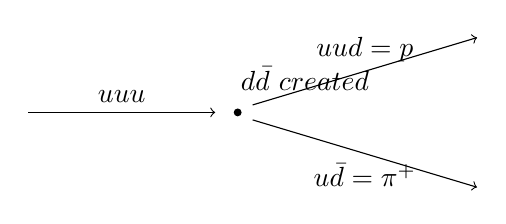
\begin{tikzpicture}[scale=0.95]
\draw[->] (-3,0) -- (-0.5,0) node[midway,above] {$uuu$};
\fill (-0.2,0) circle (1.5pt);
\draw[->] (0,0.1) -- (3,1.0) node[midway,above] {$uud=p$};
\draw[->] (0,-0.1) -- (3,-1.0) node[midway,below] {$u\bar d=\pi^+$};
\node at (0.7,0.45) {$d\bar d\ \text{created}$};
\end{tikzpicture}
\caption{Constituent regrouping in the decay \(\Delta^{++}\rightarrow p+\pi^+\).}
\end{figure}

Charge conservation is immediate:
\begin{equation}
Q(p)+Q(\pi^+)=1+1=2=Q(\Delta^{++}).
\end{equation}
The rough mass balance also permits the decay:
\begin{equation}
1200\,\mathrm{MeV}
>
940\,\mathrm{MeV}+140\,\mathrm{MeV}.
\end{equation}
There is enough energy left for kinetic energy in the final state.

All four Delta states can decay to a proton or neutron together with a pion. Their lifetimes are extremely short. An order-of-magnitude estimate is the time light takes to cross a proton:
\begin{equation}
\tau_\Delta
\sim
\frac{10^{-13}\,\mathrm{cm}}
     {10^{10}\,\mathrm{cm/s}}
\sim10^{-23}\,\mathrm{s}.
\end{equation}
They nevertheless live long enough to be identified as distinct objects produced in particle collisions.

\begin{classroomqa}
\audiencequestion{Does the written order of the \(u\) and \(d\) symbols matter in this constituent bookkeeping?\lecturetimestamp{00:48:49}}
\lecturerresponse{Not for the purpose at hand. The important information is the flavor content and the way the full quantum state is combined.}
\end{classroomqa}

\section{The Pauli Puzzle and the Need for Color}

The \(\Delta^{++}\) exposes a contradiction. It consists of three up quarks. In a spin-\(\tfrac32\) state their ordinary spins can all point in the same direction. Their isospins are also identical because they are all \(u\). If spin, flavor, and the lowest-energy spatial state were the whole description, the three quarks would be identical fermions occupying the same state. The Pauli exclusion principle forbids this.

\begin{classroomqa}
\audiencequestion{How can the repeated up quarks be fermions if they appear to occupy the same state?\lecturetimestamp{00:48:58}}
\lecturerresponse{They cannot be identical in every quantum number. The \(\Delta^{++}\) shows that quarks require an additional label beyond ordinary spin, flavor, and the spatial state. That additional label is color.}
\end{classroomqa}

The new label has three possible values:
\begin{equation}
r,\qquad g,\qquad b,
\end{equation}
called red, green, and blue. The words have nothing to do with visible color. They are arbitrary names for three internal states. Other names could have been used; what matters is that there are three distinct possibilities.

The red, green, and blue versions of a given quark flavor have the same mass and the same ordinary observable properties. They are nevertheless distinct quantum states. A \(\Delta^{++}\) can therefore contain one red \(u\), one green \(u\), and one blue \(u\), so the three fermions do not occupy the same complete state.

The six flavors are
\begin{equation}
u,\ d,\ c,\ s,\ t,\ b.
\end{equation}
This ordering is not by mass. The up quark is the lightest and the down quark comes next. The charm quark is much heavier than the strange quark, and the top quark is vastly heavier than the bottom quark. Each flavor comes in three colors. A quark therefore carries at least two distinct internal labels:
\begin{equation}
\text{flavor}\quad\text{and}\quad\text{color}.
\end{equation}

Could the three quarks have been distinguished by position or momentum instead? The Delta puzzle concerns the lowest-energy state, for which the relevant spatial and momentum structure cannot supply three distinct labels without changing the energy and symmetry properties. The missing distinction must be a new internal degree of freedom.

There is an instructive analogy with the role of spin in atomic physics. Two electrons that appear to occupy the same orbital state can still differ by their spin state. In the same structural way, quarks that agree in flavor, ordinary spin, and spatial state can differ by color.

\editorialnote{The precise historical route involving helium spectroscopy, the Pauli principle, and Uhlenbeck and Goudsmit was explicitly treated as uncertain. The analogy is retained without asserting that this was the exact chronology by which spin was discovered.}

Yoichiro Nambu was associated with recognizing that quarks required this additional degree of freedom. The physical point is independent of its name: three quark colors resolve the Pauli contradiction. The relevant exclusion principle is the Pauli principle, not the Heisenberg uncertainty principle.

\editorialnote{The precise attribution and later history of the name \emph{color} were left uncertain, so no firmer chronology is asserted here. A spoken reference to the Heisenberg uncertainty principle is corrected to the Pauli exclusion principle, as required by the surrounding fermion-statistics argument.}

The same color construction applies to the proton and neutron. Their states are not built by assigning one permanently identifiable color to each written flavor symbol. A physical baryon is a quantum superposition of the possible red, green, and blue assignments, combined with the appropriate exchange symmetries.

\begin{classroomqa}
\audiencequestion{Is color an ordinary physical property that can be measured directly?\lecturetimestamp{00:56:55}}
\lecturerresponse{The three colors have the same mass and the same ordinary properties. Their distinction is revealed relationally, through allowed combinations and collision processes. Experiments show that three distinct color states are present even though an isolated colored quark cannot be prepared for direct inspection.}
\end{classroomqa}

\begin{classroomqa}
\audiencequestion{Is color conserved?\lecturetimestamp{00:57:38}}
\lecturerresponse{Yes. Color is conserved, but the observable particles under discussion always have zero color, so it is a somewhat unusual-looking conservation law.}
\end{classroomqa}

\editorialnote{More precisely, asymptotic hadrons are color singlets. The phrase ``zero color'' is not an abelian net charge obtained by numerically adding red, green, and blue.}

\begin{classroomqa}
\audiencequestion{Does the \(uud\) proton by itself really require all three colors? It seems sufficient merely to distinguish the two \(u\) quarks.\lecturetimestamp{00:57:58}}
\lecturerresponse{That example visibly requires some additional distinction, but it does not make the number three unavoidable. The \(\Delta^{++}\), with three up quarks of parallel ordinary spin and parallel isospin, makes the need for three distinct labels unambiguous.}
\end{classroomqa}

This is why the Delta played such an important role. The proton and neutron have more complicated spin and flavor symmetries, so the contradiction can be obscured by the details of their wavefunctions. In the \(\Delta^{++}\), the conflict is immediate:
\begin{equation}
uuu,\qquad
\uparrow\uparrow\uparrow,
\qquad
\text{one lowest spatial state}.
\end{equation}
A new three-valued label is required. The existence of three color states is also confirmed independently by hadron-collision data.

A symmetry label can be meaningful even when its alternatives are equivalent in isolation. Without a chosen spatial axis, two spin directions are physically equivalent. A second object can provide a reference axis and reveal their relation. Similarly, a proton or neutron picks a direction in isospin space, and comparisons with other states reveal whether internal orientations are parallel or antiparallel. Color is subtler, but its physical content likewise appears through relations, correlations, and interaction rules rather than through visible coloring.

One could instead imagine abandoning the Pauli principle. That would require a new mathematical framework: ordinary quantum field theory classifies particles as fermions or bosons and provides no established third option that solves this problem. QCD keeps the fermionic nature of quarks and introduces color.

\begin{classroomqa}
\audiencequestion{What observable corresponds to the hidden distinction required by the Pauli principle?\lecturetimestamp{01:01:08}}
\lecturerresponse{That question is much subtler than the familiar position, momentum, or isospin observables. Its full answer requires more of the color dynamics and is deferred.}
\end{classroomqa}

\begin{classroomqa}
\audiencequestion{Was the fermionic character of quarks inferred from the spin assignments of hadrons?\lecturetimestamp{01:01:43}}
\lecturerresponse{Yes.}
\end{classroomqa}

\editorialnote{The wording of the two preceding audience questions is partly obscured. Their subjects and the brief responses are secure, but no more detailed formulation is inferred.}

\begin{classroomqa}
\audiencequestion{How can one associate a particular color with one quark in a proton?\lecturetimestamp{01:01:55}}
\lecturerresponse{One does not assign a fixed color to a permanently identifiable constituent. The proton is a quantum superposition of all allowed red, green, and blue assignments, with the spin, flavor, spatial, and color factors symmetrized or antisymmetrized appropriately. The \(\Delta^{++}\) is useful because its parallel spin and flavor structure exposes the need for color without requiring the full proton wavefunction.}
\end{classroomqa}

Color is to QCD what electric charge is to electrodynamics: it is the quantum number that controls the interaction. QCD gives a highly accurate account of experimental data from hadron collisions. The ultimate justification for the framework is that its consequences agree with experiment.

\section{Photons and Gluons}

Quarks are the fermionic matter particles of QCD, analogous in this limited respect to electrons in QED. What binds them?

In electrodynamics, an electron is a source of electromagnetic field. In particle language it emits and absorbs photons, and photon exchange produces forces between charged particles. A quark is similarly a source of the gluon field and can emit and absorb gluons.

Gluons resemble photons in several important respects. They are massless spin-one particles and have photon-like polarization states. Their momentum and polarization are ordinary dynamical properties. The crucial difference is that gluons carry color information and therefore interact with one another.

Photons carry no electric charge. At the primitive QED level, one photon does not emit another photon, and two light beams pass through one another without interacting. There are very small higher-order photon-photon interactions involving electron loops, but these are secondary effects rather than a direct photon self-coupling. In empty space, the elementary QED vertex is simply an electron emitting or absorbing a photon.

\begin{figure}[h]
\centering
\begin{tikzpicture}[scale=1.0]
\draw[->] (-2,-1) -- (0,0);
\draw[->] (0,0) -- (2,-1);
\draw[smooth] plot coordinates {
(0,0) (0.16,0.27) (0.32,0.23) (0.48,0.52)
(0.64,0.48) (0.80,0.77) (0.96,0.73)
(1.12,1.02) (1.28,0.98) (1.44,1.27)
(1.60,1.23) (1.76,1.52)
};
\node at (-1.25,-0.75) {$e^-$};
\node at (1.25,-0.75) {$e^-$};
\node at (1.95,1.62) {$\gamma$};
\fill (0,0) circle (1.5pt);
\end{tikzpicture}
\caption{Elementary QED vertex: an electron emits or absorbs a photon.}
\end{figure}

Reversing the direction of a fermion line turns the electron interpretation into a positron interpretation. Emission, absorption, and crossed positron processes are all rearrangements of this one vertex.

For bookkeeping, one can pretend that a photon has some of the properties of an electron--positron pair. The pair is electrically neutral, and aligned electron and positron spins can form total spin one. With an external interaction supplying the required energy and momentum, a photon can produce an electron--positron pair. None of this means that a photon is literally made from an electron and a positron. The fictitious-pair picture contributes little to QED itself, but its color analogue is useful in QCD.

\section{Color--Anticolor Labels for Gluons}

Represent the three color states of a quark as a column:
\begin{equation}
q=
\begin{pmatrix}
r\\
g\\
b
\end{pmatrix}.
\end{equation}
Represent the corresponding antiquark labels as a row:
\begin{equation}
\bar q=
\begin{pmatrix}
\bar r&\bar g&\bar b
\end{pmatrix}.
\end{equation}

A gluon is not a quark--antiquark bound state. Nevertheless, its color bookkeeping behaves as if it carried one color and one anticolor. The possible labels can therefore be arranged as
\begin{equation}
\begin{pmatrix}
r\bar r&r\bar g&r\bar b\\
g\bar r&g\bar g&g\bar b\\
b\bar r&b\bar g&b\bar b
\end{pmatrix}.
\end{equation}
At first sight this gives nine combinations.

\begin{classroomqa}
\audiencequestion{Are the diagonal color--anticolor entries indistinguishable?\lecturetimestamp{01:13:37}}
\lecturerresponse{Not simply. The diagonal entries are distinct; the point is that their sum is not an independent quantum state.}
\end{classroomqa}

There are actually only eight independent gluon states. The three diagonal labels are not simply indistinguishable from one another, but the particular diagonal sum
\begin{equation}
r\bar r+g\bar g+b\bar b
\end{equation}
does not furnish an additional independent gluon of QCD. The deeper explanation of this reduction is postponed. For the present color-flow arguments, it is useful to work with the nine apparent labels and remember that one diagonal combination is absent.

\section{The Quark--Gluon Vertex}

A quark can emit a gluon and emerge with either the same or a different color. If a quark enters with color \(a\) and leaves with color \(b\), the emitted gluon carries the bookkeeping label \(a\bar b\):
\begin{equation}
a\longrightarrow b+(a\bar b).
\end{equation}
For example,
\begin{equation}
r\longrightarrow g+(r\bar g).
\end{equation}
The red color line continues into the gluon, while the green line continues through the outgoing quark and reverses into an antigreen line in the gluon.

The quark need not change color. The same rule also allows
\begin{equation}
r\longrightarrow r+(r\bar r),
\end{equation}
or
\begin{equation}
r\longrightarrow b+(r\bar b).
\end{equation}

\begin{figure}[h]
\centering
\begin{tikzpicture}[scale=1.0]
\draw[->] (-2,-0.8) -- (0,0) node[midway,above] {$r$};
\draw[->] (0,0) -- (2,0.9) node[midway,above] {$g$};
\draw[smooth] plot coordinates {
(0,0) (0.20,-0.23) (0.40,-0.17) (0.60,-0.46)
(0.80,-0.40) (1.00,-0.69) (1.20,-0.63)
(1.40,-0.92) (1.60,-0.86) (1.80,-1.15)
(2.00,-1.09)
};
\node at (2.35,-1.12) {$r\bar g$};
\fill (0,0) circle (1.5pt);
\end{tikzpicture}
\caption{A red quark becomes green while emitting an \(r\bar g\) gluon.}
\end{figure}

This is one primitive building block of QCD.

\begin{classroomqa}
\audiencequestion{Can a gluon be emitted only when the quark changes color?\lecturetimestamp{01:17:15}}
\lecturerresponse{No. The outgoing quark may have the same color or a different color. In either case, the emitted gluon's color--anticolor label makes the color lines continuous.}
\end{classroomqa}

\section{The Three-Gluon Vertex}

QCD has another primitive interaction with no elementary analogue in QED. A gluon can interact directly with other gluons.

Begin with an \(r\bar b\) gluon. In color-flow language it may split as
\begin{equation}
r\bar b
\longrightarrow
r\bar g+g\bar b.
\end{equation}
The red line continues into \(r\bar g\), the antiblue line continues into \(g\bar b\), and the green-antigreen pair joins the two outgoing gluons. This gives a three-gluon vertex.

\begin{figure}[h]
\centering
\begin{tikzpicture}[scale=1.0]
\draw[smooth] plot coordinates {
(-2,0) (-1.80,0.12) (-1.60,-0.02) (-1.40,0.12)
(-1.20,-0.02) (-1.00,0.12) (-0.80,-0.02)
(-0.60,0.12) (-0.40,-0.02) (-0.20,0.12) (0,0)
};
\draw[smooth] plot coordinates {
(0,0) (0.20,0.27) (0.40,0.21) (0.60,0.50)
(0.80,0.44) (1.00,0.73) (1.20,0.67)
(1.40,0.96) (1.60,0.90) (1.80,1.19) (2.00,1.13)
};
\draw[smooth] plot coordinates {
(0,0) (0.20,-0.27) (0.40,-0.21) (0.60,-0.50)
(0.80,-0.44) (1.00,-0.73) (1.20,-0.67)
(1.40,-0.96) (1.60,-0.90) (1.80,-1.19) (2.00,-1.13)
};
\node at (-2.45,0) {$r\bar b$};
\node at (2.45,1.18) {$r\bar g$};
\node at (2.45,-1.18) {$g\bar b$};
\fill (0,0) circle (1.5pt);
\end{tikzpicture}
\caption{Three-gluon color flow: \(r\bar b\rightarrow r\bar g+g\bar b\).}
\end{figure}

There is no need to memorize every allowed combination. Follow each color line through the diagram. When a fermion line reverses its time direction, reinterpret it as the corresponding antiparticle or anticolor line.

\section{Gluon Exchange and Forces}

A gluon produces forces by being exchanged, just as a photon produces electromagnetic forces by being exchanged between charged particles.

For example, a blue quark and an antiblue antiquark can exchange a \(g\bar b\) gluon and emerge as green and antigreen. A color-flow assignment satisfying both vertices is\footnote{The net color change \(b+\bar b\longrightarrow g+\bar g\) is explicit, but the local color labels are corrected several times. The exchanged label \(g\bar b\) is reconstructed by requiring continuous color flow at both vertices.}
\begin{equation}
b+\bar b
\longrightarrow
g+\bar g.
\end{equation}
At the antiquark vertex,
\begin{equation}
\bar b\longrightarrow\bar g+(g\bar b),
\end{equation}
while at the quark vertex,
\begin{equation}
b+(g\bar b)\longrightarrow g.
\end{equation}
The exchanged gluon carries the color change from one fermion line to the other.

\begin{figure}[h]
\centering
\begin{tikzpicture}[scale=1.0]
\draw[->] (-1.8,0) -- (-1.8,-1.8) node[midway,left] {$\bar b$};
\draw[->] (-1.8,1.8) -- (-1.8,0) node[midway,left] {$\bar g$};
\draw[->] (1.8,-1.8) -- (1.8,0) node[midway,right] {$b$};
\draw[->] (1.8,0) -- (1.8,1.8) node[midway,right] {$g$};
\draw[smooth] plot coordinates {
(-1.8,0) (-1.50,0.13) (-1.20,-0.03) (-0.90,0.13)
(-0.60,-0.03) (-0.30,0.13) (0,-0.03)
(0.30,0.13) (0.60,-0.03) (0.90,0.13)
(1.20,-0.03) (1.50,0.13) (1.8,0)
};
\node at (0,0.42) {$g\bar b$};
\fill (-1.8,0) circle (1.5pt);
\fill (1.8,0) circle (1.5pt);
\end{tikzpicture}
\caption{Exchange of a \(g\bar b\) gluon changes a blue--antiblue pair into a green--antigreen pair; antiquark arrows point opposite to increasing time.}
\end{figure}

The same interaction permits forces between gluons. A consistent realization is\footnote{The lecture establishes gluon exchange between gluons and the follow-the-lines rule, but the local labels in the diagram are repeatedly revised. The displayed assignment is one consistent realization of the final rule rather than a secure transcription of every intermediate label.}
\begin{equation}
(r\bar b)+(b\bar r)
\longrightarrow
(r\bar g)+(g\bar r),
\end{equation}
with a \(g\bar b\) gluon exchanged between the two external gluons:
\begin{align}
r\bar b&\longrightarrow r\bar g+g\bar b,\\
b\bar r+g\bar b&\longrightarrow g\bar r.
\end{align}

\begin{figure}[h]
\centering
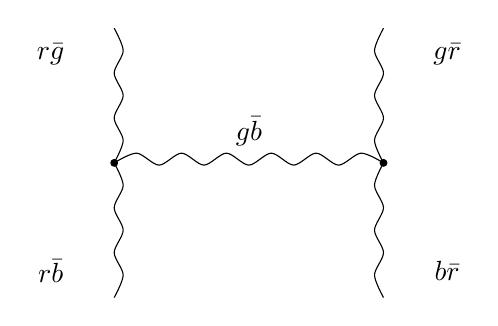
\begin{tikzpicture}[scale=0.95]
\draw[smooth] plot coordinates {
(-1.8,-1.8) (-1.68,-1.50) (-1.80,-1.20) (-1.68,-0.90)
(-1.80,-0.60) (-1.68,-0.30) (-1.8,0)
};
\draw[smooth] plot coordinates {
(-1.8,0) (-1.68,0.30) (-1.80,0.60) (-1.68,0.90)
(-1.80,1.20) (-1.68,1.50) (-1.8,1.8)
};
\draw[smooth] plot coordinates {
(1.8,-1.8) (1.68,-1.50) (1.80,-1.20) (1.68,-0.90)
(1.80,-0.60) (1.68,-0.30) (1.8,0)
};
\draw[smooth] plot coordinates {
(1.8,0) (1.68,0.30) (1.80,0.60) (1.68,0.90)
(1.80,1.20) (1.68,1.50) (1.8,1.8)
};
\draw[smooth] plot coordinates {
(-1.8,0) (-1.50,0.13) (-1.20,-0.03) (-0.90,0.13)
(-0.60,-0.03) (-0.30,0.13) (0,-0.03)
(0.30,0.13) (0.60,-0.03) (0.90,0.13)
(1.20,-0.03) (1.50,0.13) (1.8,0)
};
\node at (-2.65,-1.45) {$r\bar b$};
\node at (-2.65,1.45) {$r\bar g$};
\node at (2.65,-1.45) {$b\bar r$};
\node at (2.65,1.45) {$g\bar r$};
\node at (0,0.42) {$g\bar b$};
\fill (-1.8,0) circle (1.5pt);
\fill (1.8,0) circle (1.5pt);
\end{tikzpicture}
\caption{Exchange of a \(g\bar b\) gluon between two gluons, with each color and anticolor line continuous through the vertices.}
\end{figure}

\section{Gluon Self-Interaction and Nonlinear Fields}

Gluon self-interaction changes the character of QCD. Quarks can bind by exchanging gluons and form hadrons, but gluons can also bind by exchanging gluons. QCD can therefore contain composite objects made entirely from gluonic degrees of freedom, with no quarks. There is no corresponding elementary bound state in QED made only from photons.

The field language gives the same conclusion. Two electromagnetic waves in empty space pass through one another at the elementary level. Two gluon waves interact and deform one another. Even different portions of one gluon field configuration can exert forces on each other. The gluon field is therefore nonlinear.

\begin{classroomqa}
\audiencequestion{Must the same numbers of red, green, and blue labels appear on each side of a diagram?\lecturetimestamp{01:24:59}}
\lecturerresponse{The practical rule is to follow every color line through the diagram. That continuity is color conservation. If a fermion line turns around in time, its label becomes the corresponding antiparticle or anticolor label.}
\end{classroomqa}

\begin{classroomqa}
\audiencequestion{Are all the color and anticolor labels in the first version of the diagram consistent?\lecturetimestamp{01:26:00}}
\lecturerresponse{No. Several labels must be corrected. In a consistent assignment, the red, antiblue, and green lines each continue through the vertices, with a reversed fermion arrow interpreted as an antiparticle.}
\end{classroomqa}

\begin{classroomqa}
\audiencequestion{Is an intermediate gluon line being treated as a quark--antiquark pair?\lecturetimestamp{01:27:58}}
\lecturerresponse{Only in its color bookkeeping. A gluon is not literally a quark--antiquark composite, but it carries the corresponding color and anticolor properties.}
\end{classroomqa}

At this stage the elementary rules are compact:

\begin{itemize}
\item quarks emit and absorb gluons;
\item gluons interact directly with gluons;
\item every color and anticolor line must continue through a vertex;
\item reversing a fermion line in time changes it into the corresponding antiparticle line.
\end{itemize}

\begin{classroomqa}
\audiencequestion{Are gluons still massless when they are represented by all these color--anticolor lines?\lecturetimestamp{01:28:13}}
\lecturerresponse{Yes. Gluons remain massless. The following qualification concerns what is meant by the mass assigned to a quark inside a hadron.}
\end{classroomqa}

Confinement and the structure of hadrons come next: why isolated color is never observed and how quarks and gluons organize themselves inside composite particles. First, it is useful to clarify what is meant by the mass of a constituent quark.

\section{Probe Scale and the Meaning of Quark Mass}

Imagine a small object of mass \(m\) attached to a soft, deformable piece of material---a dangling piece of chewing gum will do. Apply a very gentle force, so slowly that the soft material has time to adjust and the entire system moves together. The measured inertia is then the inertia of the small object plus the attached material.

Now shake the small object at very high frequency. The soft material does not have time to follow the rapid motion. It remains nearly stationary while the small core responds. The measured high-frequency inertia is then much closer to \(m\) alone.

\begin{figure}[h]
\centering
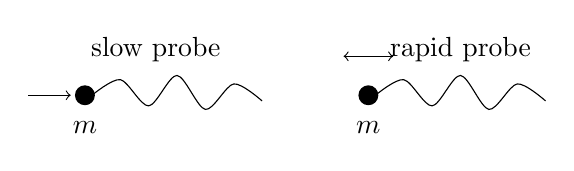
\begin{tikzpicture}[scale=0.9]
\fill (-3,0) circle (4pt);
\node at (-3,-0.45) {$m$};
\draw[smooth] plot coordinates {
(-2.9,0) (-2.5,0.22) (-2.1,-0.15) (-1.7,0.28)
(-1.3,-0.20) (-0.9,0.16) (-0.5,-0.08)
};
\draw[->] (-3.8,0) -- (-3.2,0);
\node at (-2.0,0.65) {slow probe};

\fill (1.0,0) circle (4pt);
\node at (1.0,-0.45) {$m$};
\draw[smooth] plot coordinates {
(1.1,0) (1.5,0.22) (1.9,-0.15) (2.3,0.28)
(2.7,-0.20) (3.1,0.16) (3.5,-0.08)
};
\draw[<->] (0.65,0.55) -- (1.35,0.55);
\node at (2.3,0.65) {rapid probe};
\end{tikzpicture}
\caption{A slow probe moves the core and its soft attachment together, whereas a rapid probe initially measures mainly the core response.}
\end{figure}

This is a classical analogy. The inferred mass depends on the frequency of the applied force because different parts of the system have time to participate at different frequencies.

A quark inside a hadron is surrounded by strongly interacting gluonic material and by the other constituents. If one could pull very slowly on a quark, the entire hadron would respond. The inertia encountered would then be of order the nucleon mass,
\begin{equation}
m_N\sim930\text{--}940\,\mathrm{MeV}.
\end{equation}
If the quark is struck very hard and probed over a very short time, the initial response is associated with the much smaller mass parameter conventionally assigned to a light quark, roughly
\begin{equation}
m_{u,d}\sim5\text{--}10\,\mathrm{MeV}
\end{equation}
in the estimates being used here.

Thus the phrase ``the mass of a quark'' requires a specification of the scale of the probe. A gentle, low-frequency disturbance moves the extended composite; a hard, high-frequency disturbance initially resolves a much smaller part of it. This analogy is not a derivation of renormalization, but it motivates why parameters used to describe particles depend on the frequencies and wavelengths of the interactions in which they are measured. Such scale-dependent parameters are called running parameters or running constants.

\begin{classroomqa}
\audiencequestion{Is this frequency-dependent mass merely a restatement of an uncertainty relation such as \(\Delta x\,\Delta t\)?\lecturetimestamp{01:33:32}}
\lecturerresponse{No. The example is already a classical phenomenon. A small mass attached to something soft accelerates one way under a rapid force and another way under a slow force because different amounts of the attached material have time to respond.}
\end{classroomqa}

\begin{classroomqa}
\audiencequestion{Does the earlier discussion of the electron's electric charge involve the same kind of scale dependence?\lecturetimestamp{01:34:04}}
\lecturerresponse{Yes. The general lesson is that the parameters used to describe particles depend on the frequencies and wavelengths of the interactions in which they are probed. They are called running constants.}
\end{classroomqa}

\begin{classroomqa}
\audiencequestion{Does the same qualification apply to the fractional charge assigned to a quark?\lecturetimestamp{01:34:36}}
\lecturerresponse{It does. One must define carefully what is meant by the charge of a quark. At this level it is quoted relative to the proton charge; a fuller definition is a separate discussion.}
\end{classroomqa}

\editorialnote{The fixed fractional electric-charge quantum number and the scale-dependent interaction coupling are distinct. Running of the coupling does not change the \(+\tfrac23\) or \(-\tfrac13\) flavor labels themselves.}

\begin{classroomqa}
\audiencequestion{Why does the color bookkeeping always use a quark and an antiquark? Why could two quarks not form the corresponding object?\lecturetimestamp{01:34:55}}
\lecturerresponse{That is an important question, but its answer belongs to the next discussion of allowed color combinations and confinement.}
\end{classroomqa}

\begin{classroomqa}
\audiencequestion{If individual quarks cannot be isolated, how were fractional charge, color, and the quark model inferred?\lecturetimestamp{01:35:17}}
\lecturerresponse{The picture emerged gradually from many clues together with apparent contradictions. Hadron patterns suggested quark constituents; the Delta states exposed a conflict with Fermi statistics; and the permanent confinement of quarks supplied another peculiar fact. The quark proposal appeared in the early 1960s, Nambu had an important early version of the color idea, and many physicists assembled and tested the full structure over roughly the following decade. It was not the result of one observation or one person.}
\end{classroomqa}

\begin{classroomqa}
\audiencequestion{Why are there only eight gluons rather than the nine apparent color--anticolor combinations?\lecturetimestamp{01:37:24}}
\lecturerresponse{The detailed explanation of why the diagonal sum is not an additional gluon is deferred.}
\end{classroomqa}

\begin{classroomqa}
\audiencequestion{Is this discussion of QCD ignoring electrons?\lecturetimestamp{01:37:33}}
\lecturerresponse{Yes. QCD is being isolated in the same way that a discussion of QED may temporarily ignore quarks. The separate sectors must ultimately be combined into a larger structure containing quarks, electrons, photons, and the other particles. Some parts of that larger synthesis have been accomplished and some remain incomplete. Physics often proceeds by isolating a subsystem, understanding it, and then putting the pieces back together.}
\end{classroomqa}
